%!TEX program = xelatex 
\documentclass[A4paper]{article}
\usepackage{geometry}
\geometry{left = 3cm, right = 3cm, top = 3cm, bottom = 3cm}
\usepackage[linesnumbered,ruled,longend]{algorithm2e}
\usepackage{amsmath}
\usepackage{amsfonts,amssymb}
\usepackage{blkarray}
\usepackage{booktabs}
\usepackage{dsfont}
\usepackage{enumerate}
\usepackage{epsf}
\usepackage{fontspec}
\usepackage{forest}
\usepackage[colorlinks=true,linkcolor=purple]{hyperref}
\usepackage{listings}
\usepackage{mathrsfs}
\usepackage{microtype}
\usepackage{multirow}
\usepackage{setspace}
\usepackage{tikz}
%\usepackage{indentfirst}
%\usepackage[usenames,dvipsnames]{xcolor}
\newfontfamily\Inputmono{Consolas}
\renewcommand\thesection{Question\ \arabic{section}}%\arabic{section}}
\renewcommand\thesubsection{(\arabic{subsection})}
\renewcommand\thesubsubsection{\arabic{subsubsection}.}
\newcommand{\qedhere}{$\hfill\ensuremath{\square}$}
\defaultfontfeatures{Mapping=tex-text,Scale=MatchLowercase}
\newcommand\mycommfont[1]{\ttfamily\textcolor{blue}{#1}}
\SetCommentSty{mycommfont}
%\setmainfont{Citadel Script}
%\setmainfont{Chalkboard}
\setmainfont{CMU Bright}
%\setmainfont{Apple Chancery}
\setmonofont{Optima}
\setsansfont{Optima}
%\renewcommand{\familydefault}{\sfdefault}
%\renewcommand{\footnotesize}{\sfdefault}
\setlength{\parskip}{0.25em}
\setlength{\parindent}{0em}

%%%%%%%%%%%Configurations for code%%%%%%%%%%%%%%%%%%%%%%%
\SetKwInOut{Input}{Input} 
\SetKwInOut{Output}{Output} 
\SetKwProg{Fn}{Function}{\string:}{end} 
\SetKwFunction{mstnew}{MST\_New}
\SetKwFunction{tw}{TreeWeight}
\SetKwFunction{dps}{DFS}
\SetKwFunction{con}{Is\_Connected}
\SetKwFunction{hor}{Three\_Fastest\_Horses}
%%%%%%%%%%%Here is the configurations for Code%%%%%%%%%%%

%\definecolor{mygreen}{rgb}{0,0.6,0}
%\definecolor{mygray}{rgb}{0.7,0.7,0.7}
%\definecolor{mymauve}{rgb}{0.58,0,0.82}
%\definecolor{mywhite}{rgb}{1,1,1}
%\definecolor{myblack}{rgb}{0,0,0}
%\definecolor{myblue}{RGB}{27,154,154}
%\lstset{
% backgroundcolor=\color{white}, 
% basicstyle = \footnotesize\Inputmono,       
% breakatwhitespace = false,        
% breaklines = true,                 
% captionpos = b,                    
% commentstyle = \color{mygray}\bfseries,
% extendedchars = false,             
% frame =shadowbox, 
% framerule=0.5pt,
% frameround=tttt,
% keepspaces=true,
% keywordstyle=\color{myblue}\bfseries, % keyword style
% language = Verilog,                     % the language of code
% otherkeywords={string}, 
% numbers=left, 
% numbersep=5pt,
% numberstyle=\tiny\color{mymauve},
% rulecolor=\color{black},         
% showspaces=false,  
% showstringspaces=false, 
% showtabs=false,    
% stepnumber=0,         
% stringstyle=\color{mymauve},        % string literal style
% tabsize=2,          
% title=\lstname                      
%}

%%%%%%%%%%%%%%%%%%%%%%%%%%%%%%%%%%%%%%%%%%%%

\begin{document}
%\setmainfont{Savoye LET}
%\setmainfont{Cormorant Upright}
\setmainfont{Cormorant Upright}
\renewcommand\arraystretch{1.5}


\thispagestyle{empty}

\begin{center}
\begin{large}
\begin{figure}[!htbp]
\centering

\includegraphics[width=0.7\textwidth]{Logo2.png}
\end{figure}
\hrule
\vspace*{0.25cm}
\sc{UM--SJTU Joint Institute \vspace*{0.3em}} \\ 
VE477 Intro to Algorithms\\
\end{large}
\hrulefill

\vspace*{3cm}

\begin{Large}
\sc{{Homework 3}} \\
\end{Large}
\vspace*{2cm}
\begin{large}
\sc{{Wang, Tianze\\ 515370910202}} \\
\end{large}
\end{center}
\newpage
\setmainfont{Optima}
\setmonofont{Optima}
\setsansfont{Optima}
%\tableofcontents
%\newpage
\setcounter{page}{1}
\section{Hamilton Path}
A Hamilton Path is a path that visit each vertex in a graph exactly once.
\subsection{}
Not done yet.
\subsection{}
Not done yet.
\subsection{}
\begin{algorithm}
\caption{Hamilton Algorithm}
\SetKwFunction{hc}{Hamilton}
\Input{An undirected graph $G$}
\Output{The Hamilton Path in $G$}
\Fn{\hc{$G$}}{
	L $\leftarrow$ []\;
	S $\leftarrow$ nodes with no coming edges\;
	\If{S size >1}{
		\KwRet{No result}
	}
	\If{S size == 0}{
		Reverse the direction of all edges\;
		S' $\leftarrow$ nodes with no coming edges\;
		\uIf{S' size ==0}{
			\KwRet{Exist Hamilton Path}
		}
		\Else{
			\While{$S$ $\neq  \varnothing$}{
		remove $n$ from $S$\;
		Append $n$ to tail of $L$\;
		\For{node $m$ with an edge $e$ from $n$ to $m$}{
			remove $e$ from graph.
		}
		Update $S$\;
	}
	\uIf{Graph has other edges}{
		\KwRet{No result}
	}
	\Else{
		\KwRet{L}
	}
		}

	}
	\While{$S$ $\neq  \varnothing$}{
		remove $n$ from $S$\;
		Append $n$ to tail of $L$\;
		\For{node $m$ with an edge $e$ from $n$ to $m$}{
			remove $e$ from graph.
		}
		Update $S$\;
	}
	\uIf{Graph has other edges}{
		\KwRet{No result}
	}
	\Else{
		\KwRet{L}
	}
}
\end{algorithm}
\newpage
\begin{flushleft}
\subsection{Complexity}
The complexity is a DFS with stack, and the algorithm will visit every vertex and every edge in the graph for only once, so the overall complexity is 
\[
 	\mathcal{O}(V+E)
 \] 
\end{flushleft}
\subsection{}
Linear Complexity.

\section{Critical Thinking}
\subsection{}
The answer is no. The reason is that, to be bounded by polynomial, it should have time complexity of $\mathcal{O}(n^k)$. However, in this case, for\[
	\lceil \log n \rceil !
\] 
We are not able to find a $k$ satisfying the condition since the existing factorial calculation.
\subsection{}
Yes.\\
The definition of $\log ^*$ is 
\[
	x = \left\{
	\begin{aligned}
	&0 \ \ \ & x \leq 1\\
	&1 + \log^* \log_2 x & x > 1
	\end{aligned}
	\right.
\]
And the definition of $f(x)$ to be asymptotically larger than $g(x)$ is 
\[
	\underset{x\rightarrow \infty}{lim} \frac{f(x)}{g(x)} = \infty
\]
In this problem, \[
	\begin{aligned}
	\log^* \log n & = \log^* (\frac{\log_2 n}{\log_2e} )
	\end{aligned}
\]
which means,
\[
	\log^* n -2 <\log^* \log n < \log* n -1
\]
And we can conclude
\[
	\log^* \log n = O(\log^* n)
\]
The result is then
\[
	\underset{x\rightarrow \infty}{lim} \frac{\log^* n -1}{\log\log^* n} = \underset{a\rightarrow \infty}{lim} \frac{a}{\log a} = \infty
\]
\qedhere
\subsection{}
We will only need 3 weigh.
\begin{algorithm}
\SetKwFunction{bs}{get\_ball}
\Input{8 balls with one lighter and 7 same weight}
\Output{The light weight ball}
\Fn{\bs{8 balls}}{
	Divide 8 balls into two 4-ball groups, $A_1 $, $A_2$\;
	Weigh $A_1$, $A_2$\;
	Divide lighter-weight 4 balls into two 2-ball groups, $B_1$, $B_2$\;
	Weigh $B_1$, $B_2$\;
	Weigh inside the lighter-weight group from $B_1$ and $B_2$.
	\KwRet{Lighter weight ball from previous weigh}
}
\end{algorithm}
\section{Rubik's Cube}
The Rubik's cube is a cube with 6 sides in different color, and each side is cut into 9 identical square pieces. There is an internal pivot such that enable each side to rotate, when the side is rotating, 3 adjacent square pieces that adjacent to the rotating side in all 4 adjacent sides will move with the side. To solve a Rubik's cube, all sides should be restored to same color. \\
\par \textbf{Solving Strategy 1: CFOP} A method called CFOP, which is a short spelling for Cross, First-2-layers, Orienting-the-last-layer, Permutation-last-layer. First build a cross, on a single layer, the cross should be also valid for the adjacent for side. Second, finish the bottom two layer according to formula. Third, finish upper slide, without considering the permutation of the layer.(namely the color are correct however the position may be wrong) Fourth, finish the permutation, using formula.
\par \textbf{Solving Strategy 2: Heise Method}  A method is defined in 4 steps. First, build 4 successive square-shaped blocks. 
\begin{figure}[!htbp]
\centering
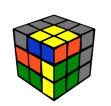
\includegraphics[width=0.1\textwidth]{HW3_pb1.png}
\end{figure}
\begin{flushleft}
Second, match the sequence and orient edges.
\end{flushleft}
\begin{figure}[!htbp]
\centering
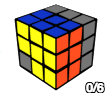
\includegraphics[width=0.1\textwidth]{HW3_pb2.png}
\end{figure}
Third, solve the remaining edges and any two corners. Fourth, solve all the corners. \\
\url{https://www.ryanheise.com/cube/heise_method.html} 
\end{document}	



















\begin{algorithm}
\caption{Hamilton Algorithm}
\SetKwFunction{hc}{Hamilton}
\Input{An undirected graph $G$}
\Output{The Hamilton Path in $G$}
\Fn{\hc{$G$}}{
	Arbitrary get a permutation of vertices in any way\;
	\For{vertices in the permutation not being adjacent}{
		Mark these vertices as break points\;
	}
	\For{All break points except for one left}{
		add edge to break points, which shall be deleted later\;
	}
	main\_break\_point $\leftarrow$ the only breakpoint\;
	main\_break\_point\_list\ $\leftarrow$ []\;
	\textbf{Append} main\_break\_point \textbf{to} main\_break\_point\_list\;
	\While{There is at least one breakpoint}{
		Cut a segment from the permutation with only one break point\;
		
		\If{All break points in main\_break\_point\_list are different from newly-created break point \textbf{and}\\
			The number of new break point to be least \textbf{or} no new breakpoint}{
				Insert it in the cycle\;
				\If{no new break point}{\textbf{break}\;}
				main\_break\_point\_list $\leftarrow$ new break point\;
				\textbf{Append} main\_break\_point \textbf{to} main\_break\_point\_list\;
			}
	}
	\KwRet{The permutation, namely the Hamilton Path}
}
\end{algorithm}
\subsection{}
The complexity is mainly decided by the updating process. Now we have the number of all possible break points to be 
\[
	(N-1)^2
\]
and each iteration, it will take polynomial time ($\mathcal{O}(N)$) computation since there is no recursive call inside iteration. The maximum cost will be visiting all the possible break points, and that will cost no more than
\[
	\mathcal{O}(N^3)
\]
So the complexity is polynomial time.
\subsection{}
It belongs to cubic time complexity.





